% ============================================================
% M3 S2 导学件·波1 臂6 片件 —— 课时13 双曲线的标准方程（2.6.1）＝批C 四片之四（母版照抄制）
% 生成：M3 成卷轮 S2 波1 臂6｜2026-09-14｜编译 cwd＝本目录（中文路径禁 \input 绝对路径）
%   xelatex main-true.tex ×2 → 含详解印本；xelatex main-false.tex ×2 → 纯题版（单源双本）
% 输入链（全只读）：题面库 课时13-2.6.1双曲线的标准方程.md（题面逐字装配）＋ -答案侧.md（值逐字回嵌）
%   ＋ 定稿/批C-课时13-2.6.1双曲线的标准方程.md（详解回嵌源，§9 补产全文区）；toolchain＝qp-m3.sty
%   （钉后版 md5 7c3930362be8a0a2bdf21bbf8ac16573，本地挂载副本，破损即停）。
% 母版体例：详见 成卷/导学件/课时01-坐标法/母版体例说明.md（结构骨架/宏用法/门谱跑法/常见坑）。
% 键账：件内 ansblock 键集 ≡ 题面库片键集 ≡ manifest 键序（21 键，零缺漏零多余）；
%   预习位零键零答案（口令④裁定前口径）；印面号 1—21＝探究 1—16＋课堂评价 17—21，
%   键↔号映射见 值台账-课时13.json。
% 括线判据（承重墙禁放宽）：估高＞8 行（chars/23 栏宽口径）→ 括线模，逐键读数入值台账；
%   其余灰底。本片括线键读数见值台账（门谱实测）。
% 观察注落实（任务令随片下发）：难2＝件13-#25 借入难位（0.4 难+档，件内§6 登记），题面照录在印、
%   【图注】以 bindp 文本行照录；简9/简10＝0913 命制入槽照录（简10 轮4回修版防 2.6.2 前引）；
%   简1 与教材习题2-4C②同文防双收（教材侧不收，案头账）；本片多选 0（原中5/6 两席 0913 置换
%   移拓展册13-拓5/拓6，正文门多选 0 合规）；逐条读数见 值台账-课时13.json「观察注落实」。
% 字形注：值行含 −（U+2212，补钉路由拉丁字体）、≠（U+2260）、±√²＜ 等常用区字形，缺字门实测见门谱读数。
% 门谱读数：见过程件 工作区/_tmpM3S2波1臂6_0914/（编译 log、门谱输出、键表）。
% ============================================================
\documentclass[fontset=none]{ctexart}
\usepackage{qp-m3}
% —— 印面逐字符号路由补钉（探针实证 0914：书宋缺 U+2212，▱ 诸字库皆缺→NSC 子块；
%     禁改 sty 本体保 md5；无 ▱/− 用件的片可整块照抄，零副作用） ——
\xeCJKDeclareCharClass{Default}{"2212}%
\setCJKfamilyfont{nscblk}[Path=C:/提示词/工作区/字替对照-0909/variantF/fonts/,BoldFont=NSC-w600.ttf]{NSC-w500.ttf}%
\xeCJKDeclareSubCJKBlock{nscblk}{"25B1}%
\newcommand{\pxparallelogram}{{\CJKfamily{nscblk}▱}}%
% —— 断行微调（纯题档/详解档三零门：CJK 胶收缩 0.01→0.05em；只动伸缩分量不动自然宽度） ——
\xeCJKsetup{CJKglue={\hskip 0.10em plus 0.08em minus 0.05em}}%
% —— 页脚件名（qp-headfoot 复用入口） ——
\renewcommand{\qpzhangming}{第二章\quad 平面解析几何}%
\renewcommand{\qpjianming}{导学件}%

\begin{document}

\zhangtitle{第二章\quad 平面解析几何}
\jietitle{2.6.1 双曲线的标准方程}
\mubiaoline
\mubiaomu{1}{理解双曲线的定义，掌握焦点在\(x\)轴、\(y\)轴上的双曲线的标准方程，会求\(a\)、\(b\)、\(c\)并判定轨迹存在性；}
\mubiaomu{2}{会依条件（焦点、过点、等轴、方程类型等）求双曲线的标准方程，能判定含参方程所表示的曲线类型；}
\mubiaomu{3}{能综合运用定义处理焦点三角形、过焦点弦周长、折线最值与圆切轨迹、实际定位等问题.}

\vspace{1.7mm}
\begin{multicols}{2}
\emergencystretch=1em

% ============================================================
% 课前预习（知识点导学填空；零键零答案——预习键位按检查口令④裁定前口径，
% \kongbai 空线＋\zhentib 判断题面形，两档等形不泄答）
% ============================================================
\huaxing{课}{前}{预}{习}{知识导学\quad 素养初识}

\zsd{一}{双曲线的定义与标准方程}

\tiaomu{1}{定义：平面内与两定点\(F_1\)、\(F_2\)的距离的\kongbai{}等于常数（小于\(|F_1F_2|\)且不为0）的点的轨迹；标准方程：焦点在\(x\)轴\kongbai{}，焦点在\(y\)轴\kongbai{}；\(a\)、\(b\)、\(c\)关系：\kongbai{}．\zhuzhu{与椭圆差号勿混：双曲线\(c^{2}=a^{2}+b^{2}\)对椭圆\(a^{2}=b^{2}+c^{2}\)；\(2a<|F_1F_2|\)才成双曲线，\(2a=|F_1F_2|\)退化为两射线，\(2a>|F_1F_2|\)或\(2a=0\)无轨迹（或为直线）.}}

\zsd{二}{依条件求标准方程·方程类型判定}

\tiaomu{1}{待定系数：先定焦点位置设标准形，由条件（过点、焦点、\(a\)、\(b\)等）列方程组；含参方程化「=1」后看两项系数的\kongbai{}判定曲线类型．\zhuzhu{焦点未定设\(mx^{2}-ny^{2}=1\)（\(mn>0\)）统一两位置；等轴双曲线\(a=b\)设\(x^{2}-y^{2}=t\)（\(t\neq 0\)）避位置讨论.}}

\zsd{三}{定义的综合应用（焦点三角形·轨迹·最值）}

\tiaomu{1}{焦点三角形：第一定义定\(2a\)，联余弦定理或勾股求面积、求高；过焦点弦与另一侧焦半径拼周长；折线差最值用「三角形两边之差小于第三边」＋取等核验．\zhuzhu{圆切轨迹族：与两定圆一内切一外切的圆心轨迹为双曲线（两支并存勿擅自限支）；轨迹题先把几何条件译成距离等式，再与\(2c\)比大小定存在性.}}

\zhenhead{判断正误(正确的打\gou{},错误的打\cha{})}

\zhentib{(1)}{双曲线\(x^{2}/4-y^{2}/9=1\)的焦点在\(x\)轴上．}

\zhentib{(2)}{平面内到两定点距离之差为常数（小于两定点间距离）的点的轨迹是双曲线．}

\zhentib{(3)}{点\(P(x_0,y_0)\)在双曲线\(x^{2}/a^{2}-y^{2}/b^{2}=1\)右支上的充要条件是\(x_0\geqslant a\)．}

\liubai[9mm]{此处书写}

% ============================================================
% 课中探究（考点探究〔例+变式〕＝练/拓槽 16 键；题后紧跟答案＝ansblock 内嵌，
% 值照答案侧逐字，详解承定稿 §9 回嵌）
% ============================================================
\huaxing{课}{中}{探}{究}{考点探究\quad 素养小结}

% ---------- 探究点一 定义辨析与轨迹探求 ----------
\tjdnr{一}{定义辨析与轨迹探求}{例\textbf{1}}{简单(知识点一)}{已知\(A\)，\(B\)是平面内的两点，且\(AB=6\)，分别判断平面内满足下列条件的动点\(P\)是否存在，并说明理由．(1)\(|PA|+|PB|=6\)；(2)\(|PA|-|PB|=6\)；(3)\(|PB|-|PA|=6\)；(4)\(|PA|+|PB|=3\)；(5)\(|PB|-|PA|=7\)．}
\xiexwei{12mm}

{\ansblockgrayfalse
\begin{ansblock}[2章-练-课时13-简1]
% ans:2章-练-课时13-简1
\ansitem{1}{(1)存在，轨迹是线段 AB；(2)存在，轨迹是以 B 为端点、指向 A 一侧反向（即线段 AB 的延长线方向）的射线；(3)存在，轨迹是以 A 为端点、沿线段 BA 延长线的射线；(4)不存在；(5)不存在}
\ansnote{详解}{记\(|AB|=6\)，对动点\(P\)总有\(|PA|+|PB|\geqslant|AB|\)（三角不等式）与\(\big||PA|-|PB|\big|\leqslant|AB|\)（两边之差小于等于第三边，等号当\(P\)、\(A\)、\(B\)共线）．(1)\(|PA|+|PB|=6=|AB|\)：等号成立当且仅当\(P\)在线段\(AB\)上，故轨迹为线段\(AB\)（椭圆定义中\(2a=2c\)的退化位）．(2)\(|PA|-|PB|=6=|AB|\)：须\(\big||PA|-|PB|\big|=|AB|\)，即\(P\)、\(A\)、\(B\)共线且\(P\)不在\(A\)、\(B\)之间；再由\(|PA|>|PB|\)知\(P\)靠\(B\)一侧，即\(P\)在射线（以\(B\)为端点、方向背离\(A\)）上，此即“线段\(AB\)的延长线”．(3)\(|PB|-|PA|=6\)：同(2)对称，\(P\)在以\(A\)为端点、背离\(B\)的射线上（“线段\(BA\)的延长线”）．(4)\(|PA|+|PB|=3<6=|AB|\)：与三角不等式矛盾，满足条件的\(P\)不存在（轨迹不存在）．(5)\(|PB|-|PA|=7>6=|AB|\)：与\(\big||PB|-|PA|\big|\leqslant|AB|\)矛盾，\(P\)不存在（轨迹不存在）．}
\end{ansblock}}

\liB{变式\textbf{2}}{简单(知识点一)}{}{已知\(F_1(-3,0)\)、\(F_2(3,0)\)，动点\(P\)满足\(\big||PF_1|-|PF_2|\big|=4\)，则\(P\)的轨迹方程为\kongbai{}．}
\xiexwei{10mm}

\begin{ansblock}[2章-练-课时13-简9]
% ans:2章-练-课时13-简9
\ansitem{2}{x²/4−y²/5＝1}
\ansnote{详解}{\(|F_1F_2|=6>4>0\)，由双曲线定义：\(2a=4\)，\(a=2\)；\(c=3\)；\(b^{2}=c^{2}-a^{2}=9-4=5\)．焦点在\(x\)轴，方程\(x^{2}/4-y^{2}/5=1\)．辨析：若差为\(6=|F_1F_2|\)，轨迹为两条射线\(y=0\)（\(x\leqslant -3\)或\(x\geqslant 3\)）；若差大于\(6\)，则无轨迹．}
\end{ansblock}

\liB{变式\textbf{3}}{简单(知识点二)}{}{已知\(x^{2}/(1-k)-y^{2}/(|k|-3)=-1\)，当\(k\)为何值时：(1)方程表示双曲线；(2)表示焦点在\(x\)轴上的双曲线；(3)表示焦点在\(y\)轴上的双曲线．}
\xiexwei{12mm}

{\ansblockgrayfalse
\begin{ansblock}[2章-练-课时13-简3]
% ans:2章-练-课时13-简3
\ansitem{3}{(1)k＜−3 或 1＜k＜3；(2)1＜k＜3；(3)k＜−3}
\ansnote{详解}{两边乘\(-1\)化为标准形：\(x^{2}/(k-1)+y^{2}/(|k|-3)=1\)（须\(k-1\neq 0\)且\(|k|-3\neq 0\)）．(1)表示双曲线当且仅当两项系数异号，即\((k-1)(|k|-3)<0\)：\(k-1>0\)且\(|k|-3<0\)，即\(k>1\)且\(-3<k<3\)，得\(1<k<3\)；\(k-1<0\)且\(|k|-3>0\)，即\(k<1\)且（\(k>3\)或\(k<-3\)），得\(k<-3\)；故\(k<-3\)或\(1<k<3\)．(2)焦点在\(x\)轴上的双曲线当且仅当\(x^{2}\)项系数为正、\(y^{2}\)项为负：\(k-1>0\)且\(|k|-3<0\)，得\(1<k<3\)．(3)焦点在\(y\)轴上的双曲线当且仅当\(y^{2}\)项系数为正、\(x^{2}\)项为负：\(|k|-3>0\)且\(k-1<0\)，得\(k<-3\)（\(k>3\)与\(k<1\)无交）．}
\end{ansblock}}

\xiaojie{①识别：以定义判存在性、判轨迹族（双曲线、射线、线段、无轨迹）与含参方程定型的题，判归本题型.}
\bindp {\kaishu ②操作：第一定义三查——差的绝对值、\(2a\)与\(2c\)比大小、焦点位置定实轴所在轴；含参方程两边化「=1」看系数符号定曲线类型.}
\bindp {\kaishu ③收束：退化位（\(2a=2c\)、\(2a>2c\)、\(2a=0\)）逐一交代；两解取舍须定支核验（近焦侧\(\geqslant c-a\)、远焦侧\(\geqslant c+a\)）不可省.}

% ---------- 探究点二 依条件求标准方程 ----------
\tjdnr{二}{依条件求标准方程}{例\textbf{4}}{简单(知识点二)}{求适合下列条件的双曲线的标准方程：(1)经过点\((\sqrt{6},0)\)，\((3,2)\)；(2)焦点为\((0,-5)\)，\((0,5)\)，经过点\((4\sqrt{3}/3,\ 2\sqrt{3})\)；(3)\(a=b\)，经过点\((3,-1)\)；(4)经过\((3,-4\sqrt{2})\)和\((9/4,5)\)两点．}
\xiexwei{12mm}

{\ansblockgrayfalse
\begin{ansblock}[2章-练-课时13-简4]
% ans:2章-练-课时13-简4
\ansitem{4}{(1)x²/6 − y²/8 ＝1；(2)y²/9 − x²/16 ＝1；(3)x²/8 − y²/8 ＝1；(4)y²/16 − x²/9 ＝1}
\ansnote{详解}{(1)点\((\sqrt{6},0)\)在\(x\)轴上且在曲线上，故焦点在\(x\)轴、该点即右顶点，\(a^{2}=6\)；设\(x^{2}/6-y^{2}/b^{2}=1\)，代\((3,2)\)：\(9/6-4/b^{2}=1\)，即\(4/b^{2}=1/2\)，\(b^{2}=8\)，得\(x^{2}/6-y^{2}/8=1\)（核验\(9/6-4/8=3/2-1/2=1\)成立）．(2)焦点在\(y\)轴、\(c=5\)．设\(P(4\sqrt{3}/3,2\sqrt{3})\)，到两焦点\((0,\pm 5)\)的距离平方：\(|PF_1|^{2}=(4\sqrt{3}/3)^{2}+(2\sqrt{3}-5)^{2}=16/3+37-20\sqrt{3}=(10-3\sqrt{3})^{2}/3\)，故\(|PF_1|=10\sqrt{3}/3-3\)；\(|PF_2|^{2}=(10+3\sqrt{3})^{2}/3\)，故\(|PF_2|=10\sqrt{3}/3+3\)；于是\(2a=\big||PF_2|-|PF_1|\big|=6\)，即\(a=3\)、\(b^{2}=c^{2}-a^{2}=25-9=16\)，得\(y^{2}/9-x^{2}/16=1\)；回代\(P\)：\(12/9-(16/3)/16=4/3-1/3=1\)成立（焦点在\(y\)轴成立）．(3)\(a=b\)为等轴双曲线，两轴取向皆可能，设\(x^{2}-y^{2}=t\)（\(t\neq 0\)），代\((3,-1)\)：\(t=9-1=8>0\)，得\(x^{2}-y^{2}=8\)，即\(x^{2}/8-y^{2}/8=1\)．(4)焦点位置未定，设\(mx^{2}-ny^{2}=1\)（\(mn>0\)），代入两点：\(9m-32n=1\)、\((81/16)m-25n=1\)，由第一式\(m=(1+32n)/9\)，代第二式\((9/16)(1+32n)-25n=1\)，即\(9/16+18n-25n=1\)，\(-7n=7/16\)，\(n=-1/16\)、\(m=-1/9\)，方程为\(-x^{2}/9+y^{2}/16=1\)，即\(y^{2}/16-x^{2}/9=1\)（回代\((9/4,5)\)：\(25/16-(81/16)/9=25/16-9/16=1\)成立）．}
\end{ansblock}}

\liB{变式\textbf{5}}{简单(知识点二)}{}{已知双曲线的标准方程形如\(x^{2}/a^{2}-y^{2}/b^{2}=1\)（\(a>0\)，\(b>0\)），且\(2a=6\)、\(2b=8\)，求该双曲线的标准方程、焦点坐标与离心率（\(e=c/a\)）．}
\xiexwei{12mm}

\begin{ansblock}[2章-练-课时13-简10]
% ans:2章-练-课时13-简10
\ansitem{5}{x²/9−y²/16＝1；焦点 (±5,0)；e=5/3}
\ansnote{详解}{\(2a=6\)即\(a=3\)；\(2b=8\)即\(b=4\)；\(c^{2}=a^{2}+b^{2}=9+16=25\)，\(c=5\)．故标准方程\(x^{2}/9-y^{2}/16=1\)，焦点\((\pm 5,0)\)，\(e=c/a=5/3\)．}
\end{ansblock}

\xiaojie{①识别：给焦点/过点/等轴/双点等条件求标准方程，判归本题型.}
\bindp {\kaishu ②操作：先定焦点位置设标准形，待定系数列方程组；焦点未定设\(mx^{2}-ny^{2}=1\)（\(mn>0\)），等轴设\(x^{2}-y^{2}=t\)（\(t\neq 0\)）一步到位.}
\bindp {\kaishu ③收束：所求方程逐点回代检验；两焦点距离差与\(2a\)核对，防位置设错.}

% ---------- 探究点三 焦点三角形·周长与最值 ----------
\tjdnr{三}{焦点三角形·周长与最值}{例\textbf{6}}{简单(知识点三)}{双曲线\(x^{2}/25-y^{2}/23=1\)的两个焦点为\(F_1\)，\(F_2\)，双曲线上一点\(P\)到\(F_1\)的距离为8，则点\(P\)到\(F_2\)的距离为　　\nobreak(\kongwei)}

\bindopt {\fontsize{10.5pt}{\qpTJgLeadLiti}\selectfont \makebox[\dimexpr0.5\linewidth-1em\relax][l]{A．2或12}\makebox[\dimexpr0.5\linewidth-1em\relax][l]{B．2或18}\par}

\bindopt {\fontsize{10.5pt}{\qpTJgLeadLiti}\selectfont \makebox[\dimexpr0.5\linewidth-1em\relax][l]{C．18}\makebox[\dimexpr0.5\linewidth-1em\relax][l]{D．2}\par}

{\ansblockgrayfalse
\begin{ansblock}[2章-练-课时13-简2]
% ans:2章-练-课时13-简2
\ansitem{6}{C}
\ansnote{详解}{\(a^{2}=25\)、\(b^{2}=23\)，即\(a=5\)、\(2a=10\)，\(c^{2}=48\)、\(c=4\sqrt{3}\)．由定义\(\big||PF_2|-|PF_1|\big|=2a=10\)，即\(\big||PF_2|-8\big|=10\)，得\(|PF_2|=18\)或\(|PF_2|=-2\)（距离非负，舍），故\(|PF_2|=18\)．（存在性核验：\(c-a=4\sqrt{3}-5\approx 1.93\)、\(c+a\approx 11.93\)；\(|PF_1|=8\in[c-a,c+a)\)只能对应\(P\)在左支，此时\(|PF_2|=|PF_1|+2a=18\geqslant c+a\)成立，与选项A、B中“2”所设的右支情形（须\(|PF_2|\geqslant c-a\)且\(|PF_1|\geqslant c+a\)）不合，故不取双解．）故选：C．}
\end{ansblock}}

\liB{变式\textbf{7}}{简单(知识点三)}{}{双曲线\(x^{2}/a^{2}-y^{2}/b^{2}=1\)（\(a>0\)，\(b>0\)）过焦点\(F_1\)的弦\(AB\)，\(A\)、\(B\)两点在同一支上且长为\(m\)，另一焦点为\(F_2\)，则\(\triangle ABF_2\)的周长为　　\nobreak(\kongwei)}

\bindopt {\fontsize{10.5pt}{\qpTJgLeadLiti}\selectfont \makebox[\dimexpr0.5\linewidth-1em\relax][l]{A．\(4a\)}\makebox[\dimexpr0.5\linewidth-1em\relax][l]{B．\(4a-m\)}\par}

\bindopt {\fontsize{10.5pt}{\qpTJgLeadLiti}\selectfont \makebox[\dimexpr0.5\linewidth-1em\relax][l]{C．\(4a+2m\)}\makebox[\dimexpr0.5\linewidth-1em\relax][l]{D．\(4a-2m\)}\par}

\begin{ansblock}[2章-练-课时13-简5]
% ans:2章-练-课时13-简5
\ansitem{7}{C}
\ansnote{详解}{\(A\)、\(B\)在同一支上，由定义\(|AF_2|-|AF_1|=2a\)、\(|BF_2|-|BF_1|=2a\)（该支上的点到另一焦点较远，故取此号），两式相加：\((|AF_2|+|BF_2|)-(|AF_1|+|BF_1|)=4a\)．又弦\(AB\)过焦点\(F_1\)，\(F_1\)在\(A\)、\(B\)之间（焦点在该支围成的开口内），故\(|AF_1|+|BF_1|=|AB|=m\)，于是\(|AF_2|+|BF_2|=4a+m\)，\(\triangle ABF_2\)的周长\(=|AF_2|+|BF_2|+|AB|=4a+m+m=4a+2m\)．故选：C．}
\end{ansblock}

\liB{变式\textbf{8}}{简单(知识点三)}{}{已知\(F\)为双曲线\(C\)：\(x^{2}/9-y^{2}/16=1\)的左焦点，\(P\)，\(Q\)为双曲线\(C\)右支上的点，若\(|PQ|\)的长等于虚轴长的2倍，点\(A(5,0)\)在线段\(PQ\)上，则\(\triangle PFQ\)的周长为　　\nobreak(\kongwei)}

\bindopt {\fontsize{10.5pt}{\qpTJgLeadLiti}\selectfont \makebox[\dimexpr0.25\linewidth-1em\relax][l]{A．28}\makebox[\dimexpr0.25\linewidth-1em\relax][l]{B．36}\makebox[\dimexpr0.25\linewidth-1em\relax][l]{C．44}\makebox[\dimexpr0.25\linewidth-1em\relax][l]{D．48}\par}

{\ansblockgrayfalse
\begin{ansblock}[2章-练-课时13-简6]
% ans:2章-练-课时13-简6
\ansitem{8}{C}
\ansnote{详解}{\(a^{2}=9\)、\(b^{2}=16\)，即\(a=3\)、\(b=4\)，\(c^{2}=a^{2}+b^{2}=25\)、\(c=5\)，故左焦点\(F(-5,0)\)，虚轴长\(2b=8\)，\(|PQ|=2\times 8=16\)．点\(A(5,0)\)正是右焦点\(F'\)，且\(A\)在线段\(PQ\)上，故\(|PF|-|PA|=|PF|-|PF'|=2a=6\)（\(P\)在右支），同理\(|QF|-|QA|=6\)，两式相加：\(|PF|+|QF|=12+(|PA|+|QA|)=12+|PQ|=12+16=28\)，所以\(\triangle PFQ\)的周长\(=|PF|+|QF|+|PQ|=28+16=44\)．故选：C．}
\end{ansblock}}

\liB{变式\textbf{9}}{简单(知识点三)}{}{已知双曲线\(x^{2}/(3-m)-y^{2}/m=1\)（\(0<m<3\)）的左、右焦点分别为\(F_1\)，\(F_2\)，点\(P\)在双曲线的右支上，\(O\)为坐标原点，\(\angle PF_1F_2=30^{\circ}\)，\(|OP|=\frac{1}{2}|F_1F_2|\)，则\(m\)的值为　　\nobreak(\kongwei)}

\bindopt {\fontsize{10.5pt}{\qpTJgLeadLiti}\selectfont \makebox[\dimexpr0.5\linewidth-1em\relax][l]{A．\(\sqrt{3}/2\)}\makebox[\dimexpr0.5\linewidth-1em\relax][l]{B．\(3\sqrt{3}/2\)}\par}

\bindopt {\fontsize{10.5pt}{\qpTJgLeadLiti}\selectfont \makebox[\dimexpr0.5\linewidth-1em\relax][l]{C．\(1\)}\makebox[\dimexpr0.5\linewidth-1em\relax][l]{D．\(2\)}\par}

{\ansblockgrayfalse
\begin{ansblock}[2章-练-课时13-简7]
% ans:2章-练-课时13-简7
\ansitem{9}{B}
\ansnote{详解}{\(a^{2}=3-m\)、\(b^{2}=m\)（\(0<m<3\)保证两项均正、焦点在\(x\)轴），\(c^{2}=a^{2}+b^{2}=3\)，即\(c=\sqrt{3}\)、\(|F_1F_2|=2\sqrt{3}\)．\(|OP|=\frac{1}{2}|F_1F_2|=\sqrt{3}=|OF_1|=|OF_2|\)，即\(P\)到线段\(F_1F_2\)中点\(O\)的距离等于该线段的一半，故\(P\)在以\(F_1F_2\)为直径的圆上，\(\angle F_1PF_2=90^{\circ}\)（直径所对圆周角为直角）．在直角\(\triangle F_1PF_2\)中，\(\angle PF_1F_2=30^{\circ}\)，故\(|PF_2|=|F_1F_2|\sin 30^{\circ}=2\sqrt{3}\times\frac{1}{2}=\sqrt{3}\)，\(|PF_1|=|F_1F_2|\cos 30^{\circ}=2\sqrt{3}\times\frac{\sqrt{3}}{2}=3\)．\(P\)在右支上，由定义\(|PF_1|-|PF_2|=2a\)：\(3-\sqrt{3}=2\sqrt{3-m}\)，即\(\sqrt{3-m}=(3-\sqrt{3})/2\)，\(3-m=(9-6\sqrt{3}+3)/4=3-\frac{3\sqrt{3}}{2}\)，得\(m=\frac{3\sqrt{3}}{2}\)．（核验\(0<m<3\)：\(3\sqrt{3}/2\approx 2.598<3\)成立；此时\(a^{2}=3-m\approx 0.402>0\)成立，\(2a=3-\sqrt{3}=|PF_1|-|PF_2|\)成立．）故选：B．}
\end{ansblock}}

\liB{变式\textbf{10}}{简单(知识点三)}{}{已知\(F\)是双曲线\(x^{2}/4-y^{2}/12=1\)的左焦点，点\(A(1,4)\)，\(P\)是双曲线右支上的动点，则\(|PF|+|PA|\)的最小值为　　\nobreak(\kongwei)}

\bindopt {\fontsize{10.5pt}{\qpTJgLeadLiti}\selectfont \makebox[\dimexpr0.25\linewidth-1em\relax][l]{A．9}\makebox[\dimexpr0.25\linewidth-1em\relax][l]{B．5}\makebox[\dimexpr0.25\linewidth-1em\relax][l]{C．8}\makebox[\dimexpr0.25\linewidth-1em\relax][l]{D．4}\par}

{\ansblockgrayfalse
\begin{ansblock}[2章-练-课时13-简8]
% ans:2章-练-课时13-简8
\ansitem{10}{A}
\ansnote{详解}{\(a^{2}=4\)、\(b^{2}=12\)，即\(a=2\)、\(c^{2}=16\)、\(c=4\)，故左焦点\(F(-4,0)\)、右焦点\(F'(4,0)\)．\(P\)在右支上，由定义\(|PF|-|PF'|=2a=4\)，即\(|PF|=|PF'|+4\)，于是\(|PF|+|PA|=|PF'|+|PA|+4\geqslant|AF'|+4\)（三角不等式），\(|AF'|=\sqrt{(1-4)^{2}+4^{2}}=\sqrt{25}=5\)，故\(|PF|+|PA|\geqslant 5+4=9\)．取等核验：须\(P\)在线段\(AF'\)上，联立直线\(AF'\)（过\(A(1,4)\)、\(F'(4,0)\)，方程\(y=(16-4x)/3\)）与右支\(x^{2}/4-y^{2}/12=1\)（\(x\geqslant 2\)）得\(11x^{2}+128x-364=0\)，解得\(x=26/11\)（另一根\(-14\)舍），\(26/11\approx 2.36\in[2,4]\)，对应\(y=24/11\)，交点\((26/11,24/11)\)确实落在线段\(AF'\)上且在右支上，故等号可取，最小值为9．故选：A．}
\end{ansblock}}

\liB{变式\textbf{11}}{中档(知识点三)}{}{已知\(F_1(-4,0)\)、\(F_2(4,0)\)是双曲线\(C\)：\(x^{2}/m-y^{2}/4=1\)（\(m>0\)）的两个焦点，点\(M\)是双曲线\(C\)上一点，且\(\angle F_1MF_2=60^{\circ}\)，求\(\triangle F_1MF_2\)的面积．}
\xiexwei{12mm}

{\ansblockgrayfalse
\begin{ansblock}[2章-练-课时13-中1]
% ans:2章-练-课时13-中1
\ansitem{11}{4√3}
\ansnote{详解}{焦点\((\pm 4,0)\)即\(c=4\)、\(c^{2}=16\)；又\(c^{2}=m+4\)，即\(m=12\)，故\(a^{2}=12\)、\(a=2\sqrt{3}\)、\(2a=4\sqrt{3}\)．设\(|MF_1|=t_1\)、\(|MF_2|=t_2\)，由定义\(|t_1-t_2|=2a=4\sqrt{3}\)，平方得\(t_1^{2}+t_2^{2}-2t_1t_2=48\)……①在\(\triangle F_1MF_2\)中用余弦定理：\(t_1^{2}+t_2^{2}-2t_1t_2\cos 60^{\circ}=|F_1F_2|^{2}=64\)，即\(t_1^{2}+t_2^{2}-t_1t_2=64\)……②②\(-\)①得\(t_1t_2=64-48=16\)，所以\(S=\frac{1}{2}t_1t_2\sin 60^{\circ}=\frac{1}{2}\times 16\times\frac{\sqrt{3}}{2}=4\sqrt{3}\)．}
\end{ansblock}}

\liB{变式\textbf{12}}{中档(知识点三)}{}{双曲线\(x^{2}/9-y^{2}/16=1\)的两个焦点为\(F_1\)，\(F_2\)，点\(P\)在双曲线上，若\(PF_1\perp PF_2\)，则点\(P\)到\(x\)轴的距离为\kongbai{}．}
\xiexwei{10mm}

{\ansblockgrayfalse
\begin{ansblock}[2章-练-课时13-中2]
% ans:2章-练-课时13-中2
\ansitem{12}{16/5}
\ansnote{详解}{\(a^{2}=9\)、\(b^{2}=16\)，即\(c^{2}=25\)、\(c=5\)、\(2a=6\)、\(|F_1F_2|=10\)．设\(|PF_1|=m\)、\(|PF_2|=n\)，由定义\(\big||PF_1|-|PF_2|\big|=2a=6\)，勾股（\(PF_1\perp PF_2\)）\(m^{2}+n^{2}=|F_1F_2|^{2}=100\)，两式并立：\((m-n)^{2}=m^{2}+n^{2}-2mn\)，即\(36=100-2mn\)，得\(mn=32\)．\(\triangle PF_1F_2\)的面积既等于\(\frac{1}{2}mn\)（直角边互乘），又等于\(\frac{1}{2}|F_1F_2|\cdot h\)（以焦轴为底、\(h\)为\(P\)到\(x\)轴的距离）：\(\frac{1}{2}\times 32=\frac{1}{2}\times 10\times h\)，即\(16=5h\)，得\(h=16/5\)．（存在性核验：由\(m-n=\pm 6\)、\(mn=32\)得\((m+n)^{2}=100+64=164\)，\(m+n=2\sqrt{41}\)，故\(\{m,n\}=\{\sqrt{41}+3,\sqrt{41}-3\}\approx\{9.4,3.4\}\)，两值均正且平方和为\(2(41+9)=100\)成立；与双曲线上焦半径的取值范围（近焦点侧\(\geqslant c-a=2\)、远焦点侧\(\geqslant c+a=8\)）比对：\(9.4\geqslant 8\)配远侧、\(3.4\geqslant 2\)配近侧成立，故满足垂直条件的点\(P\)确实存在．）所以点\(P\)到\(x\)轴的距离为\(16/5\)．}
\end{ansblock}}

\liB{变式\textbf{13}}{中档(知识点三)}{}{已知平面上定点\(A(-5,0)\)和\(B(8,4)\)，又\(P\)点为双曲线\(x^{2}/16-y^{2}/9=1\)右支上的动点，则\(|PA|-|PB|\)的最大值为　　\nobreak(\kongwei)}

\bindopt {\fontsize{10.5pt}{\qpTJgLeadLiti}\selectfont \makebox[\dimexpr0.25\linewidth-1em\relax][l]{A．8}\makebox[\dimexpr0.25\linewidth-1em\relax][l]{B．10}\makebox[\dimexpr0.25\linewidth-1em\relax][l]{C．11}\makebox[\dimexpr0.25\linewidth-1em\relax][l]{D．13}\par}

{\ansblockgrayfalse
\begin{ansblock}[2章-练-课时13-中3]
% ans:2章-练-课时13-中3
\ansitem{13}{D}
\ansnote{详解}{\(a^{2}=16\)、\(b^{2}=9\)，即\(c^{2}=25\)、\(c=5\)，故\(A(-5,0)\)正是左焦点，记右焦点\(F(5,0)\)．\(P\)在右支上，由定义\(|PA|-|PF|=2a=8\)，即\(|PA|=|PF|+8\)，于是\(|PA|-|PB|=8+(|PF|-|PB|)\leqslant 8+|BF|\)（三角形两边之差小于第三边），\(|BF|=\sqrt{(8-5)^{2}+(4-0)^{2}}=\sqrt{25}=5\)，故\(|PA|-|PB|\leqslant 13\)．取等核验：须\(B\)在线段\(PF\)上，即\(P\)在射线\(F\to B\)的延长方向上；该射线参数式\((5+3s,4s)\)（\(s>0\)时经\(B\)，对应\(s=1\)），代入\(9x^{2}-16y^{2}=144\)得\(175s^{2}-270s-81=0\)，正根\(s=9/5>1\)，对应\(P(52/5,36/5)\)（核验\(9\times(52/5)^{2}-16\times(36/5)^{2}=(24336-20736)/25=144\)成立，且\(x=52/5\geqslant 4\)在右支上成立），故等号可取，最大值为13．故选：D．}
\end{ansblock}}

\xiaojie{①识别：焦点三角形（周长、面积、求高、直角逆求）、过焦点弦拼周长、焦半径折线最值，判归本题型.}
\bindp {\kaishu ②操作：第一定义给\(2a\)转移焦半径；焦点三角形联余弦定理或勾股；折线和/差最值用三角形不等式并做取等核验（联立定交点）.}
\bindp {\kaishu ③收束：定义转移后符号按支别定（同支取正差、异支取负）；取等点须回代确认在曲线上且在线段上.}

% ---------- 探究点四 轨迹构形与压轴应用 ----------
\tjdnr{四}{轨迹构形与压轴应用}{例\textbf{14}}{中档(知识点三)}{已知动圆\(M\)与两圆\((x+3)^{2}+y^{2}=4\)，\((x-3)^{2}+y^{2}=4\)中的一个内切，另一个外切，则动圆\(M\)的圆心\(M\)的轨迹方程为\kongbai{}．}
\xiexwei{10mm}

{\ansblockgrayfalse
\begin{ansblock}[2章-练-课时13-中4]
% ans:2章-练-课时13-中4
\ansitem{14}{x²/4 − y²/5 ＝1}
\ansnote{详解}{记\(F_1(-3,0)\)、\(F_2(3,0)\)，两定圆半径均为2，\(|F_1F_2|=6\)．设动圆\(M\)半径为\(r\)．情形一（与圆\(F_1\)内切、与圆\(F_2\)外切）：\(|MF_1|=r-2\)或\(2-r\)；\(|MF_2|=r+2\)．若\(|MF_1|=2-r\)，则\(|MF_1|+|MF_2|=4<|F_1F_2|=6\)，不可能（三角不等式），故\(|MF_1|=r-2\)（须\(r\geqslant 2\)），此时\(|MF_2|-|MF_1|=4\)；情形二（与圆\(F_1\)外切、与圆\(F_2\)内切）：同理\(|MF_1|=r+2\)、\(|MF_2|=r-2\)，\(|MF_1|-|MF_2|=4\)；（动圆含入定圆内的情形如上所验均导致\(|MF_1|+|MF_2|=4<6\)，故皆不出现）合写为\(\big||MF_1|-|MF_2|\big|=4<|F_1F_2|=6\)，由双曲线定义，\(M\)的轨迹是以\(F_1\)、\(F_2\)为焦点的双曲线（情形一给左支、情形二给右支，两支并存），\(2a=4\)、\(2c=6\)，即\(a=2\)、\(c=3\)、\(b^{2}=c^{2}-a^{2}=9-4=5\)，轨迹方程为\(x^{2}/4-y^{2}/5=1\)．}
\end{ansblock}}

\liB{变式\textbf{15}}{难(知识点三)}{}{已知具有公共焦点\(F_1\)，\(F_2\)的椭圆\(C_1\)与双曲线\(C_2\)在第一象限的交点为\(P\)，若\(\angle F_1PF_2=\pi/2\)，椭圆\(C_1\)与双曲线\(C_2\)的离心率分别记作\(e_1\)，\(e_2\)，则\(4e_1^{2}+e_2^{2}\)的最小值为\kongbai{}．}
\xiexwei{10mm}

{\ansblockgrayfalse
\begin{ansblock}[2章-练-课时13-难1]
% ans:2章-练-课时13-难1
\ansitem{15}{9/2}
\ansnote{详解}{设公共半焦距为\(c\)，椭圆长半轴\(a_1\)、双曲线实半轴\(a_2\)，记\(m=|PF_1|\)、\(n=|PF_2|\)．由椭圆定义\(m+n=2a_1\)、双曲线定义\(|m-n|=2a_2\)，又\(\angle F_1PF_2=90^{\circ}\)得\(m^{2}+n^{2}=4c^{2}\)；将前两式分别平方：\((m+n)^{2}+(m-n)^{2}=2(m^{2}+n^{2})\)，即\(4a_1^{2}+4a_2^{2}=2\times 4c^{2}\)，故\(a_1^{2}+a_2^{2}=2c^{2}\)，两边除\(c^{2}\)：\(1/e_1^{2}+1/e_2^{2}=2\)……①于是\(4e_1^{2}+e_2^{2}=\frac{1}{2}(1/e_1^{2}+1/e_2^{2})(4e_1^{2}+e_2^{2})=\frac{1}{2}\bigl[4+e_2^{2}/e_1^{2}+4e_1^{2}/e_2^{2}+1\bigr]=\frac{1}{2}\bigl[5+e_2^{2}/e_1^{2}+4e_1^{2}/e_2^{2}\bigr]\geqslant\frac{1}{2}\bigl[5+2\sqrt{(e_2^{2}/e_1^{2})\cdot(4e_1^{2}/e_2^{2})}\bigr]=\frac{1}{2}(5+4)=9/2\)（基本不等式）．取等条件：\(e_2^{2}/e_1^{2}=4e_1^{2}/e_2^{2}\)，即\(e_2^{2}=2e_1^{2}\)，代①：\(1/e_1^{2}+1/(2e_1^{2})=2\)，即\(3/(2e_1^{2})=2\)，得\(e_1^{2}=3/4\)、\(e_2^{2}=3/2\)，即\(e_1=\sqrt{3}/2\in(0,1)\)成立（椭圆）、\(e_2=\sqrt{6}/2\in(1,\sqrt{2})\)成立（双曲线），且\(a_1=c/e_1=2c/\sqrt{3}>c\)、\(a_2=c/e_2=\sqrt{2/3}\,c<c\)均合要求；故\(4e_1^{2}+e_2^{2}\)的最小值为\(9/2\)．}
\end{ansblock}}

\liB{变式\textbf{16}}{难(知识点三)}{}{2018年世界人工智能大会已于2018年9月在徐汇西岸举行，某高校的志愿者服务小组受大会展示项目的启发，会后决定开发一款“猫捉老鼠”的游戏，如图：\(A\)、\(B\)两个信号源相距10米，\(O\)是\(AB\)的中点，过\(O\)点的直线\(l\)与直线\(AB\)的夹角为\(45^{\circ}\)，机器猫在直线\(l\)上运动，机器鼠的运动轨迹始终满足：接收到\(A\)点的信号比接收到\(B\)点的信号晚\(8/v_0\)秒（注：信号每秒传播\(v_0\)米）．在时刻\(t_0\)时，测得机器鼠距离\(O\)点为4米．(1)以\(O\)为原点、直线\(AB\)为\(x\)轴建立平面直角坐标系（如图），求时刻\(t_0\)时机器鼠所在位置的坐标；(2)游戏设定：机器鼠在距离直线\(l\)不超过1.5米的区域运动时，有“被抓”的风险．如果机器鼠保持目前的运动轨迹不变，是否有“被抓”风险？}
\ansfig{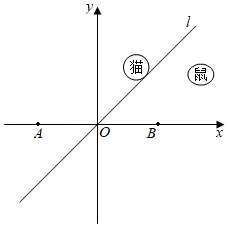
\includegraphics[width=36mm]{figs/13-难2.png}}
\xiexwei{12mm}

{\ansblockgrayfalse
\begin{ansblock}[2章-练-课时13-难2]
% ans:2章-练-课时13-难2
\ansitem{16}{(1)(4,0)；(2)没有"被抓"的风险}
\ansnote{详解}{(1)设机器鼠位置为\(P\)，声音传播时间差为距离差除以\(v_0\)：\(|PA|/v_0-|PB|/v_0=8/v_0\)，即\(|PA|-|PB|=8\)（米），而\(|AB|=10\)，\(8<10\)，由双曲线定义\(P\)的轨迹是以\(A\)、\(B\)为焦点的双曲线中靠\(B\)的一支（右支）：\(2a=8\)、\(2c=10\)，即\(a=4\)、\(c=5\)、\(b^{2}=c^{2}-a^{2}=9\)，轨迹方程\(x^{2}/16-y^{2}/9=1\)（\(x\geqslant 4\)）．时刻\(t_0\)有\(|OP|=4\)：对右支上的点\(x\geqslant 4\)，故\(|OP|=\sqrt{x^{2}+y^{2}}\geqslant x\geqslant 4\)，等号仅当\(x=4\)且\(y=0\)，即顶点\((4,0)\)，所以\(t_0\)时机器鼠所在位置坐标为\((4,0)\)．(2)直线\(l\)：\(y=x\)，设与其平行的直线\(l_1\)：\(y=x+m\)与右支相切．代入\(9x^{2}-16y^{2}=144\)：\(9x^{2}-16(x+m)^{2}=144\)，即\(7x^{2}+32mx+16m^{2}+144=0\)，\(\Delta=(32m)^{2}-4\times 7\times(16m^{2}+144)=1024m^{2}-448m^{2}-4032=576m^{2}-4032=0\)，得\(m^{2}=7\)，切点横坐标\(x=-32m/(2\times 7)=-16m/7\)，要在右支须\(x\geqslant 4\)，故取\(m=-\sqrt{7}\)（此时\(x=16\sqrt{7}/7\approx 6.05\geqslant 4\)成立；\(m=+\sqrt{7}\)的切点在左支，舍），即与右支相切且最“靠向”\(l\)的平行线为\(l_1\)：\(y=x-\sqrt{7}\)，切点\(T(16\sqrt{7}/7,9\sqrt{7}/7)\)即右支上到\(l\)最近的点．两平行线\(y=x\)与\(y=x-\sqrt{7}\)的距离\(d=|\sqrt{7}|/\sqrt{1+1}=\sqrt{14}/2\approx 1.87\)（米）\(>1.5\)，（且当\(|m|<\sqrt{7}\)时\(\Delta<0\)，即形如\(y=x+m\)的直线与双曲线无公共点，右支整体落在\(x-y\geqslant\sqrt{7}\)的一侧，故此距离确为最小值而非极值假象）所以机器鼠到直线\(l\)的最小距离为\(\sqrt{14}/2\approx 1.87\)米，大于1.5米，没有“被抓”的风险．}
\end{ansblock}}

\xiaojie{①识别：圆切轨迹（一内切一外切）、共焦点跨曲线最值、信号时差定位等轨迹构形与压轴应用，判归本题型.}
\bindp {\kaishu ②操作：圆切问题分内外切列式、剔含入定圆的伪情形，合并为差的绝对值定值；跨曲线共焦点用双定义联立消元；应用题先建系、把时间差译成距离差.}
\bindp {\kaishu ③收束：两支并存勿擅自限支；最值取等条件与存在性核验随题载明防假解.}

% ============================================================
% 课堂评价 G5（恒5＝3单选+2填空＝导槽 G1~G5；ketang 新制顺排可跨栏，禁 vbox 装栏）
% 印面号 17—21；多选门：本片正文多选 0 合规
% ============================================================
\begin{ketang}{本组共5题（第17—21题），17—19为单选，20—21为填空．}

\jiancestem{{\fontsize{11.4pt}{14pt}\selectfont\heihao {\numboldjian 17}．}\hspace{4.1mm}\tieside{简单(知识点一)}\hspace{2.2mm}已知双曲线\(x^{2}/16-y^{2}/48=1\)的左、右焦点分别为\(F_1\)，\(F_2\)，点\(P\)是该双曲线上的一点，且\(|PF_1|=10\)，则\(|PF_2|=\)　　\nobreak(\kongwei)}

\bindopt {\fontsize{10.5pt}{\qpTJgLeadPingjia}\selectfont \makebox[\dimexpr0.5\linewidth-1em\relax][l]{A．2或18}\makebox[\dimexpr0.5\linewidth-1em\relax][l]{B．2}\par}

\bindopt {\fontsize{10.5pt}{\qpTJgLeadPingjia}\selectfont \makebox[\dimexpr0.5\linewidth-1em\relax][l]{C．18}\makebox[\dimexpr0.5\linewidth-1em\relax][l]{D．4}\par}

{\ansblockgrayfalse
\begin{ansblock}[2章-导-课时13-G1]
% ans:2章-导-课时13-G1
\ansitem{17}{C}
\ansnote{详解}{\(a^{2}=16\)、\(b^{2}=48\)，即\(a=4\)，\(c^{2}=a^{2}+b^{2}=64\)、\(c=8\)，故\(a+c=12\)、\(c-a=4\)．先定支：若\(P\)在右支上，则\(|PF_1|\geqslant a+c=12\)（右支上的点到左焦点的距离以右顶点处最小，为\(a+c\)），与\(|PF_1|=10\)矛盾；所以\(P\)在左支上，左支上\(|PF_2|>|PF_1|\)，由定义\(|PF_2|-|PF_1|=2a=8\)，得\(|PF_2|=10+8=18\)．（另一解2的来源是误按“\(|10-|PF_2||=8\)”取\(|PF_2|=2\)，但此时\(P\)须在右支且\(|PF_2|\geqslant c-a=4\)，不合，舍．）故选：C．}
\end{ansblock}}

\jiancestem{{\fontsize{11.4pt}{14pt}\selectfont\heihao {\numboldjian 18}．}\hspace{4.1mm}\tieside{简单(知识点三)}\hspace{2.2mm}一动圆\(P\)过定点\(M(-4,0)\)，且与已知圆\(N\)：\((x-4)^{2}+y^{2}=16\)相切，则动圆\(P\)的轨迹方程是　　\nobreak(\kongwei)}

\lxopt{A．\(x^{2}/4-y^{2}/12=1\)（\(x\geqslant 2\)）}

\lxopt{B．\(x^{2}/4-y^{2}/12=1\)（\(x\leqslant 2\)）}

\lxopt{C．\(y^{2}/4-x^{2}/12=1\)}

\lxopt{D．\(x^{2}/4-y^{2}/12=1\)}

{\ansblockgrayfalse
\begin{ansblock}[2章-导-课时13-G2]
% ans:2章-导-课时13-G2
\ansitem{18}{D}
\ansnote{详解}{设动圆\(P\)的半径为\(r\)，则\(|PM|=r\)；圆\(N\)的圆心\(N(4,0)\)、半径4，且\(|MN|=8\)．两圆相切分三种位置：①外切\(|PN|=r+4\)；②圆\(N\)在动圆内（内切）\(|PN|=r-4\)（须\(r\geqslant 4\)）；③动圆在圆\(N\)内（内切）\(|PN|=4-r\)．情形③不可能：此时\(|PM|+|PN|=r+4-r=4<|MN|=8\)，与三角形两边之和不小于第三边矛盾（也即\(M\)在圆\(N\)外，动圆既然过\(M\)就不能整个含在圆\(N\)内）．情形①：\(|PN|-|PM|=4\)；情形②：\(|PM|-|PN|=4\)．合写即\(\big||PN|-|PM|\big|=4<|MN|=8\)，由双曲线定义，\(P\)的轨迹是以\(M\)、\(N\)为焦点的双曲线，\(2a=4\)、\(2c=8\)，即\(a=2\)、\(c=4\)、\(b^{2}=c^{2}-a^{2}=12\)，且两种切法都能实现（在双曲线上任取一点\(P\)，取\(r=|PM|\)即可作出满足条件的动圆），故两支并存、不加\(x\)的限制，轨迹方程为\(x^{2}/4-y^{2}/12=1\)．故选：D．}
\end{ansblock}}

\jiancestem{{\fontsize{11.4pt}{14pt}\selectfont\heihao {\numboldjian 19}．}\hspace{4.1mm}\tieside{简单(知识点三)}\hspace{2.2mm}已知定点\(F_1(-2,0)\)、\(F_2(2,0)\)，\(N\)是圆\(O\)：\(x^{2}+y^{2}=1\)上任意一点，点\(F_1\)关于点\(N\)的对称点为\(M\)，线段\(F_1M\)的中垂线与直线\(F_2M\)相交于点\(P\)，则点\(P\)的轨迹是　　\nobreak(\kongwei)}

\bindopt {\fontsize{10.5pt}{\qpTJgLeadPingjia}\selectfont \makebox[\dimexpr0.5\linewidth-1em\relax][l]{A．椭圆}\makebox[\dimexpr0.5\linewidth-1em\relax][l]{B．双曲线}\par}

\bindopt {\fontsize{10.5pt}{\qpTJgLeadPingjia}\selectfont \makebox[\dimexpr0.5\linewidth-1em\relax][l]{C．抛物线}\makebox[\dimexpr0.5\linewidth-1em\relax][l]{D．圆}\par}

{\ansblockgrayfalse
\begin{ansblock}[2章-导-课时13-G3]
% ans:2章-导-课时13-G3
\ansitem{19}{B}
\ansnote{详解}{\(N\)是\(F_1M\)的中点（对称关系）、\(O\)是\(F_1F_2\)的中点，故\(ON\)是\(\triangle MF_1F_2\)的中位线，即\(|MF_2|=2|ON|=2\)（\(N\)在单位圆上）．\(P\)在\(F_1M\)的垂直平分线上，即\(|PF_1|=|PM|\)；又\(P\)在直线\(F_2M\)上，故\(P\)、\(M\)、\(F_2\)三点共线，于是\(\big||PF_2|-|PF_1|\big|=\big||PF_2|-|PM|\big|=|MF_2|=2<|F_1F_2|=4\)，由双曲线定义，\(P\)的轨迹是以\(F_1\)、\(F_2\)为焦点的双曲线（\(2a=2\)、\(2c=4\)，即\(x^{2}-y^{2}/3=1\)）．故选：B．}
\end{ansblock}}

\jiancestem{{\fontsize{11.4pt}{14pt}\selectfont\heihao {\numboldjian 20}．}\hspace{4.1mm}\tieside{简单(知识点二)}\hspace{2.2mm}若三个点\((-2,1)\)，\((-2,3)\)，\((2,-1)\)中恰有两个点在双曲线\(C\)：\(x^{2}/a^{2}-y^{2}=1\)（\(a>0\)）上，则\(a=\)\kongbai{}．}
\xiexwei{10mm}

{\ansblockgrayfalse
\begin{ansblock}[2章-导-课时13-G4]
% ans:2章-导-课时13-G4
\ansitem{20}{√2}
\ansnote{详解}{把三点代入\(x^{2}/a^{2}-y^{2}\)的值：\((-2,1)\)与\((2,-1)\)都得\(4/a^{2}-1\)，\((-2,3)\)得\(4/a^{2}-9\)．先试\((-2,3)\)在\(C\)上：\(4/a^{2}-9=1\)，即\(a^{2}=2/5\)，此时另两点处的值\(4/a^{2}-1=10-1=9\neq 1\)，即只有1个点在\(C\)上，与“恰有两个”矛盾，故\((-2,3)\)不在\(C\)上．于是恰有的两个点只能是\((-2,1)\)与\((2,-1)\)（两点关于原点对称，双曲线关于原点中心对称，故同属\(C\)成立），由\(4/a^{2}-1=1\)，即\(a^{2}=2\)，得\(a=\sqrt{2}\)（\(a>0\)）．（回代核验：\(a^{2}=2\)时\(4/2-1=1\)成立，两点在\(C\)上；\(4/2-9=-7\neq 1\)成立，第三点不在，恰两个成立．）}
\end{ansblock}}

\jiancestem{{\fontsize{11.4pt}{14pt}\selectfont\heihao {\numboldjian 21}．}\hspace{4.1mm}\tieside{简单(知识点三)}\hspace{2.2mm}在\(\triangle ABC\)中，\(B(-3,0)\)，\(C(3,0)\)，直线\(AB\)，\(AC\)的斜率之积为\(16/9\)，求顶点\(A\)的轨迹方程．}
\xiexwei{12mm}

{\ansblockgrayfalse
\begin{ansblock}[2章-导-课时13-G5]
% ans:2章-导-课时13-G5
\ansitem{21}{x²/9 − y²/16 ＝1 (x≠±3)}
\ansnote{详解}{设\(A(x,y)\)，则两斜率存在须\(x\neq\pm 3\)（\(x=\pm 3\)时\(A\)与\(B\)或\(C\)的横坐标相同，直线\(AB\)或\(AC\)垂直于\(x\)轴，斜率不存在，且\(A\)与\(B\)或\(C\)重合不成三角形），\(k_{AB}=y/(x+3)\)、\(k_{AC}=y/(x-3)\)，由题意\(y^{2}/[(x+3)(x-3)]=16/9\)，即\(y^{2}/(x^{2}-9)=16/9\)，去分母：\(9y^{2}=16(x^{2}-9)\)，即\(16x^{2}-9y^{2}=144\)，得\(x^{2}/9-y^{2}/16=1\)．该双曲线上\(x^{2}\geqslant 9\)，等号只在顶点\((\pm 3,0)\)，而这两点使\(A\)与\(B\)、\(C\)重合（三角形退化），故除去\(x=\pm 3\)两点，即\(x\neq\pm 3\)（此时自动满足\(|x|>3\)，两斜率均存在成立）．所以顶点\(A\)的轨迹方程为\(x^{2}/9-y^{2}/16=1\)（\(x\neq\pm 3\)）．}
\end{ansblock}}

\end{ketang}

% ---- 尾块（\tailfill 置 \end{multicols} 前；无参＝内容尾随框，件侧不擅自定高） ----
\tailfill

\end{multicols}
\end{document}
